\section{Implementation}
\label{gacomphs19:sec:implementation}

We built the game as a web app based on the \textit{Flask}\footnote{\url{https://pypi.org/project/Flask/}} framework for \textit{Python}\footnote{\url{https://www.python.org/}}. The architecture as shown in \Cref{gacomphs19:fig:architecture} consists of a backend handling the game logic, the communication with the front end as well as the interfacing with the database. The communication is handled with a JSON-based API.

\begin{figure}[!]
	\centering
	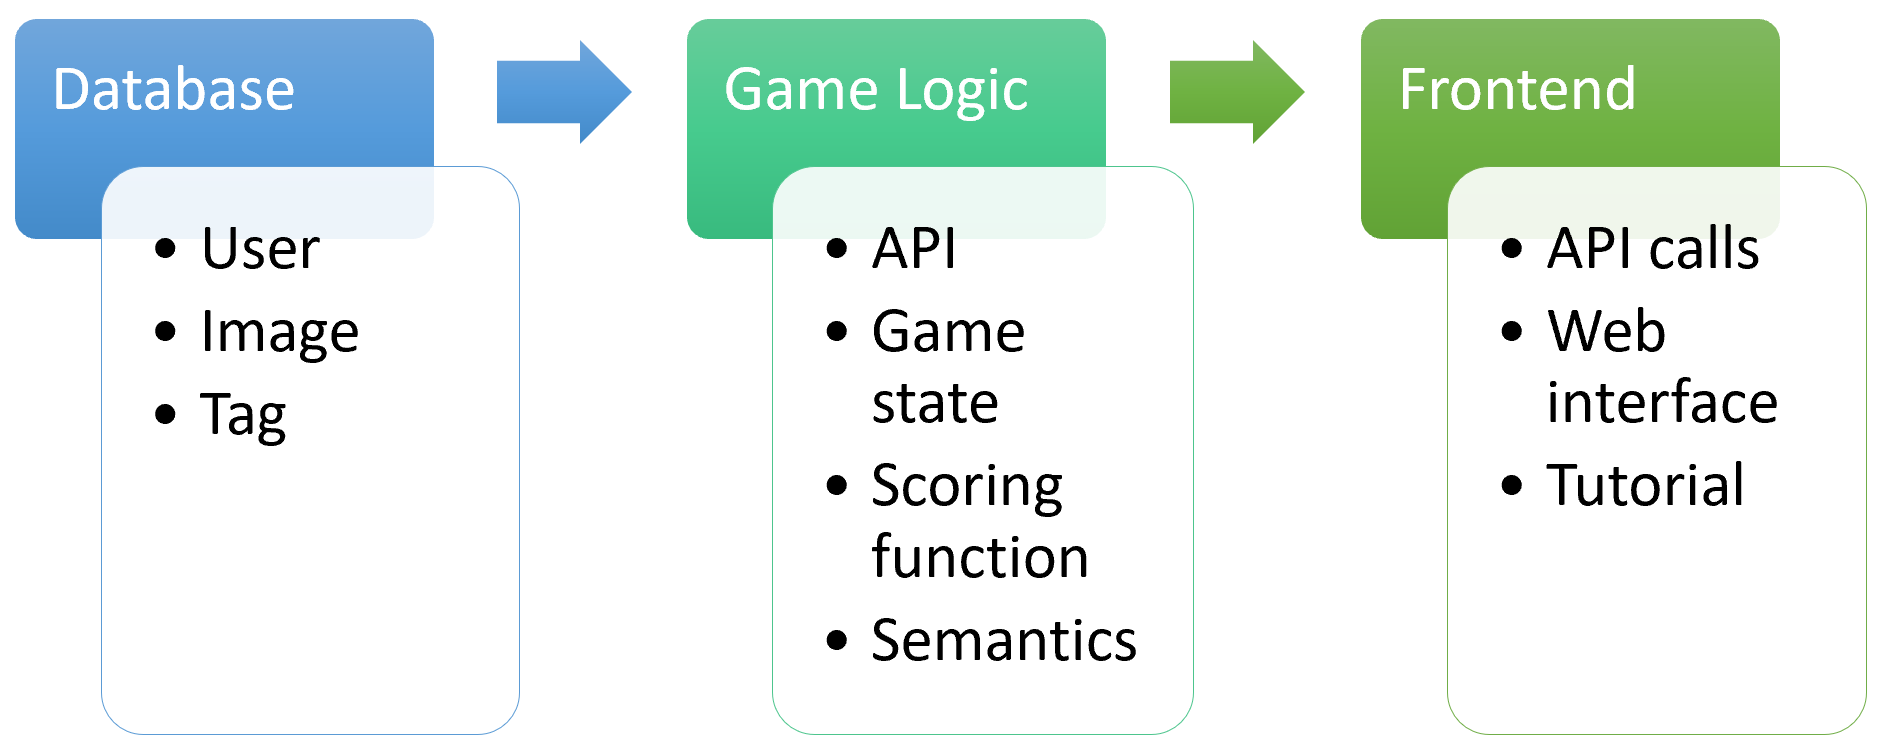
\includegraphics[width=\textwidth]{gacomphs19-architecture.png}
	\caption{architecture of the game}
	\label{gacomphs19:fig:architecture}
\end{figure}

\subsection{Game Logic}
\label{gacomphs19:sec:implementation:game}

The most interesting parts of the game are the linguistics features. The rest is fairly straightforward and connects to the database.

\subsubsection{Linguistics}
\label{gacomphs19:sec:implementation:linguistics}
The suggestion is first translated to English, if necessary. This is handled by \textit{Googletrans}\footnote{\url{https://pypi.org/project/googletrans/}}, this already provides spell checking for foreign languages.
Simple typos in English tags are fixed using \textit{SpellChecker}\footnote{\url{https://pyspellchecker.readthedocs.io/}}. We use the \textit{NLTK}\footnote{\url{https://pypi.org/project/nltk/}} library for stemming, lemmatizing and finding synonyms. If the the tag was translated, it is translated into its original language and if the tag is accepted by the game, the user is notified which word was accepted. This process can be seen in \Cref{gacomphs19:fig:semanticpipeline}.

\begin{figure}[tb]
	\centering
	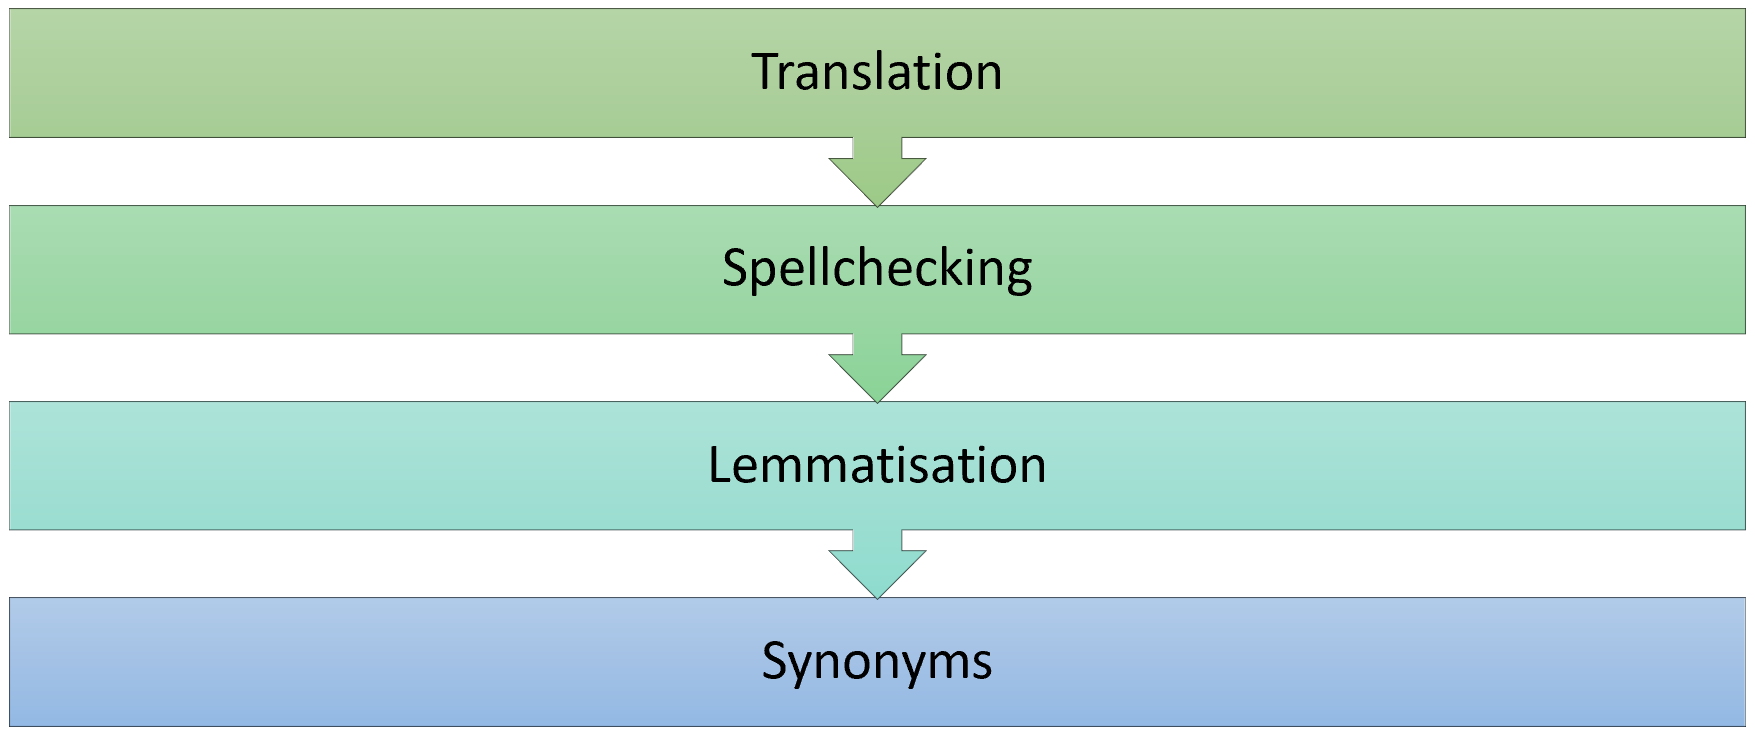
\includegraphics[width=\textwidth]{gacomphs19-semantics_pipeline.png}
	\caption{semantics pipeline}
	\label{gacomphs19:fig:semanticpipeline}
\end{figure}

\subsection{Database}
\label{gacomphs19:sec:implementation:database}
\textit{Flask-SQLAlchemy}\footnote{\url{https://flask-sqlalchemy.palletsprojects.com/}} provides an interface for common database systems. \textit{PostgreSQL}, \textit{MariaDB} and \textit{SQLite} are all compatible.
Together with \textit{Flask-Migrate} we defined a relational schema that contains entries for users, images and tags. We store the relation between users and images to ensure, that they are not shown an image twice in classic mode. The relation between tags and images is stored together with their frequency and quality.

\subsection{Login}
\label{gacomphs19:sec:implementation:login}
\textit{Flask-Login}\footnote{\url{https://flask-login.readthedocs.io/}} guarantees a stable user handling, while the current sessions are stored with \textit{Flask-Session}\footnote{\url{https://pythonhosted.org/Flask-Session/}}. This allows us to support various session backends, like Redis, Memcached, Database or filesystem based. The credentials are hashed with \textit{Flask-Bcrypt}\footnote{\url{https://flask-bcrypt.readthedocs.io/}} and the forms are XSRF protected by \textit{Flask-WTF}\footnote{\url{https://flask-wtf.readthedocs.io/}}. The way XSRF protection works is described in \cite{4198791}.

During the sign up we made a client side request to the Have I Been Pwned\footnote{\url{https://haveibeenpwned.com/API/v3\#PwnedPasswords}} API and give feedback if a match is found.

\subsection{User Interface}
\label{gacomphs19:sec:implementation:UI}

The user interface uses web technologies. Specifically, its design is built on Google's Material Design in the form of Material Design Lite\footnote{\url{https://getmdl.io/}}.

The interface has adaptive/responsive features to look okay on a variety of screen sizes, e.g. desktop formats or smart phones. The desktop GUI is shown in \Cref{gacomphs19:fig:guiclassicdesktop}, the mobile GUI in \Cref{gacomphs19:fig:guiclassicmobile}.
The markup is rendered with \textit{Jinja2} templates.



\begin{figure}[!]
\centering
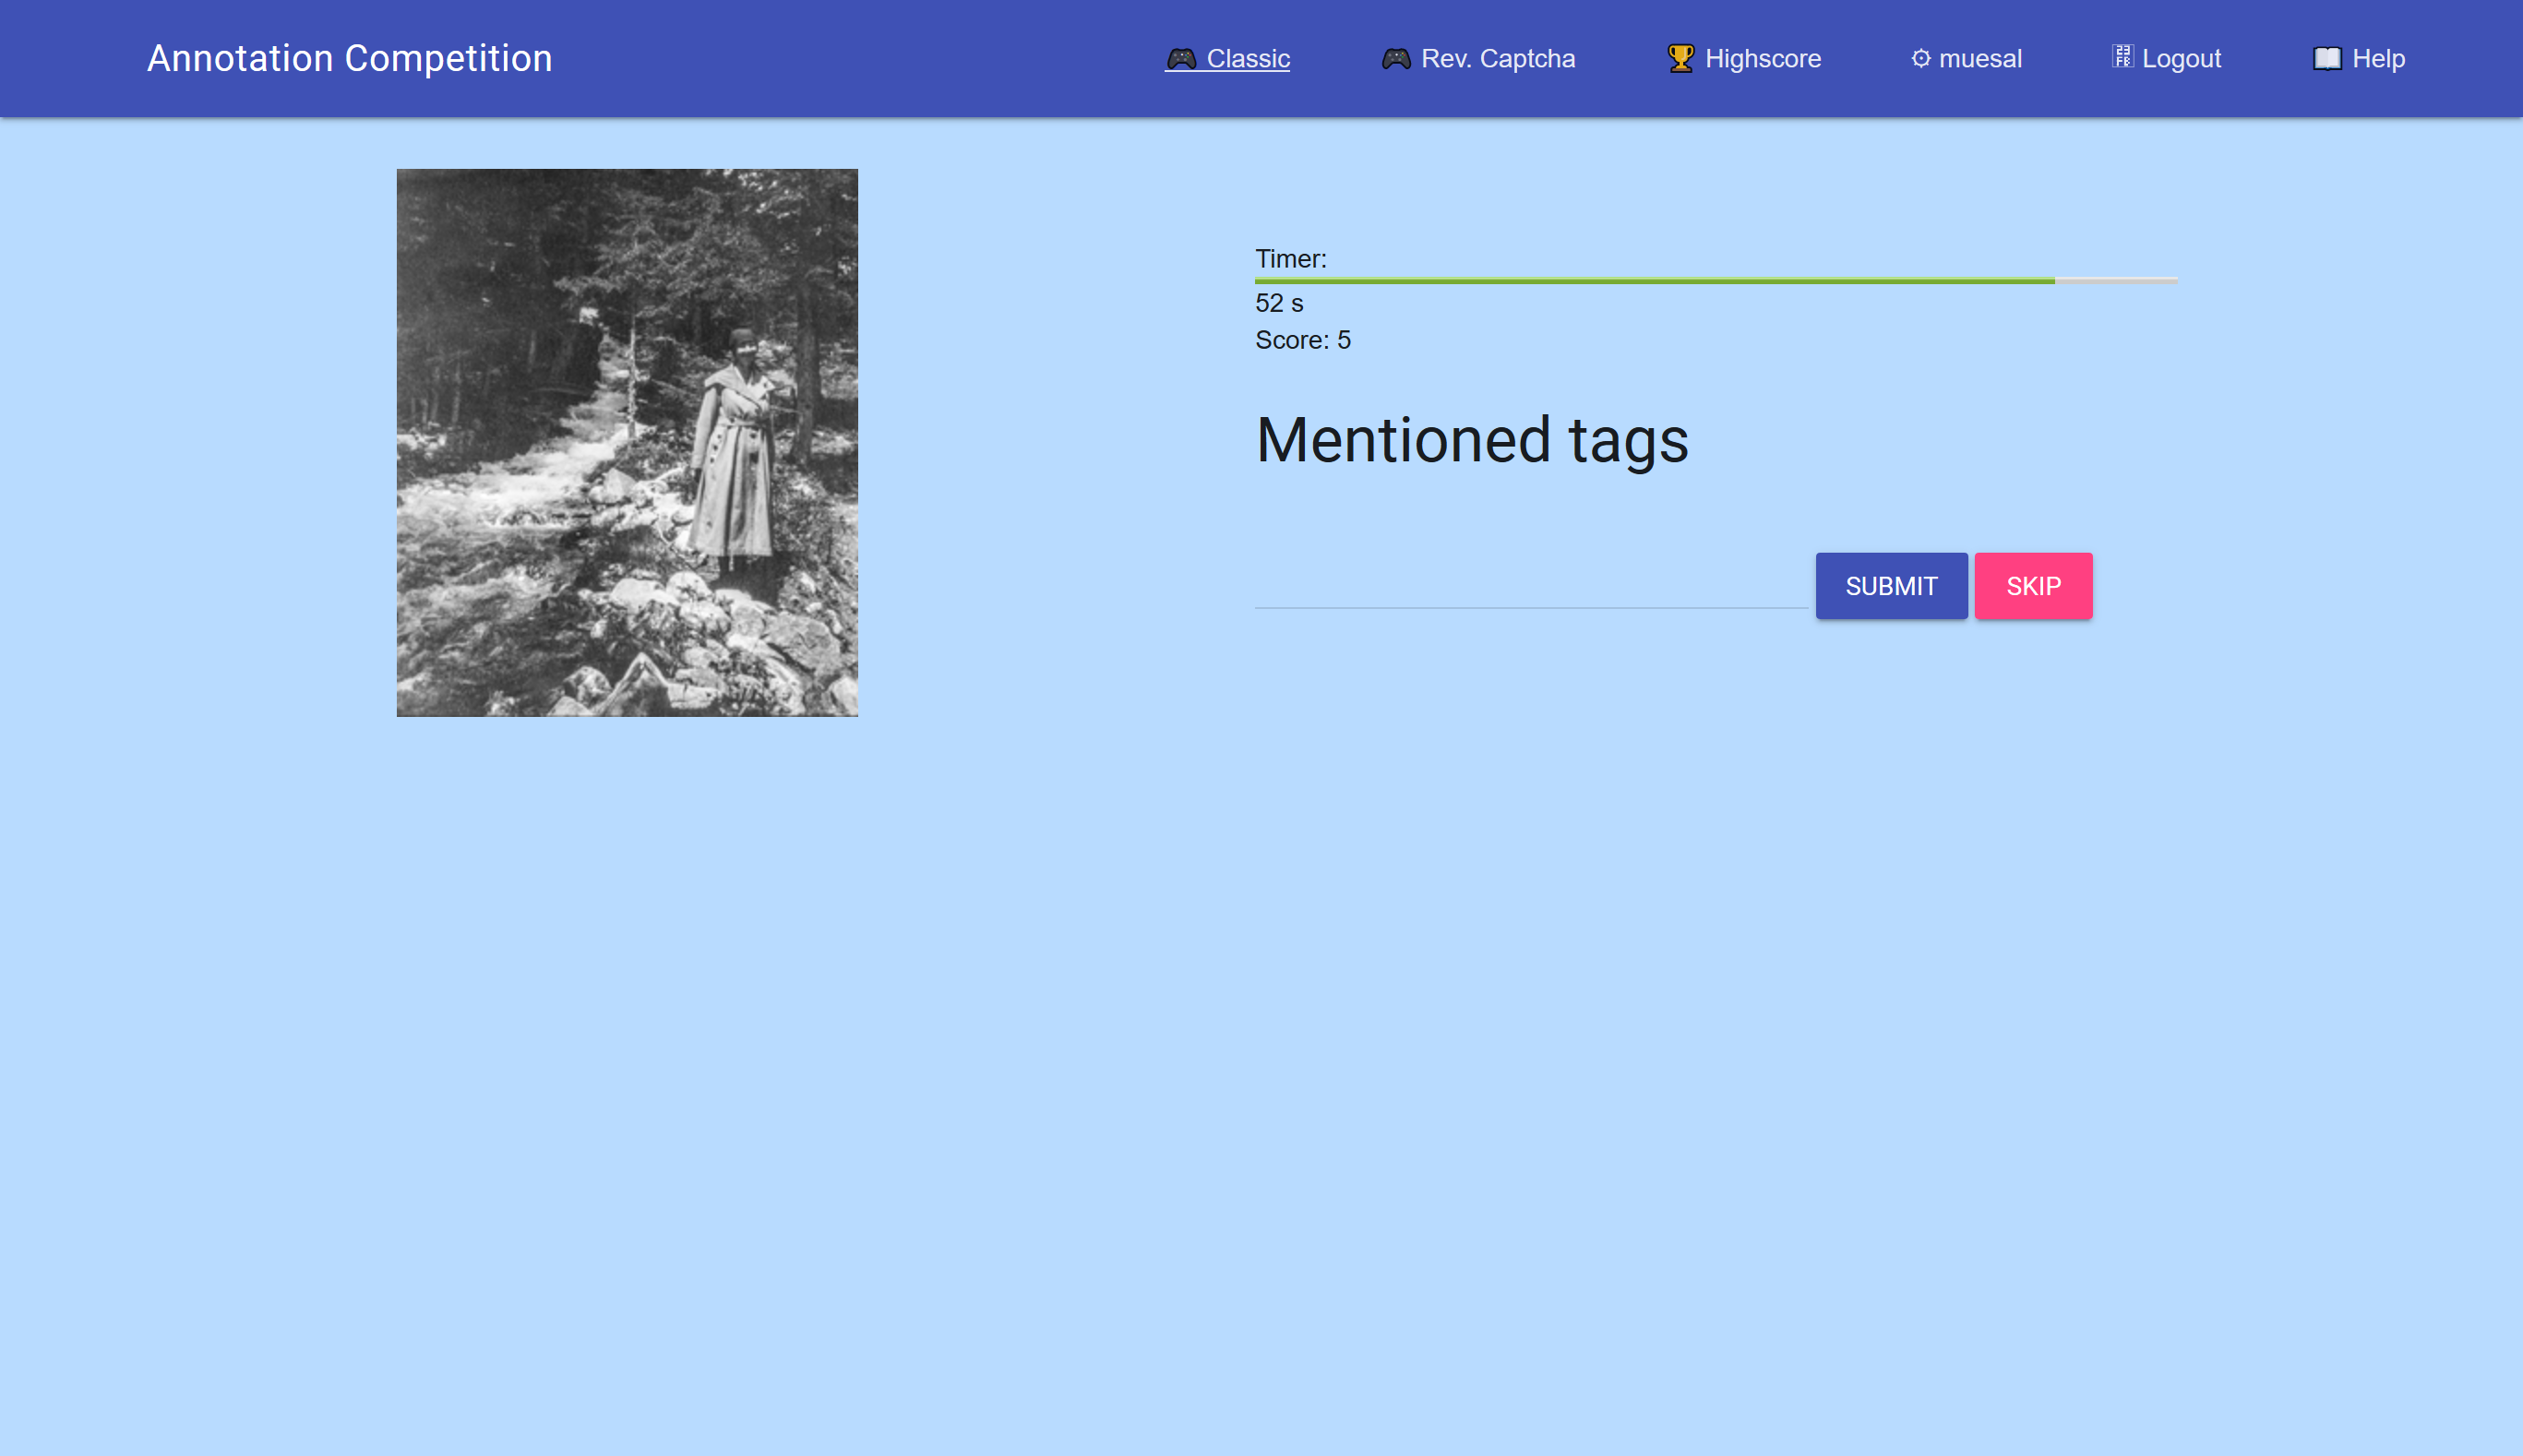
\includegraphics[width=\textwidth]{gacomphs19-classic.png}
\caption{GUI for desktop screens}
\label{gacomphs19:fig:guiclassicdesktop}
\end{figure}


\begin{figure}[!]
\centering
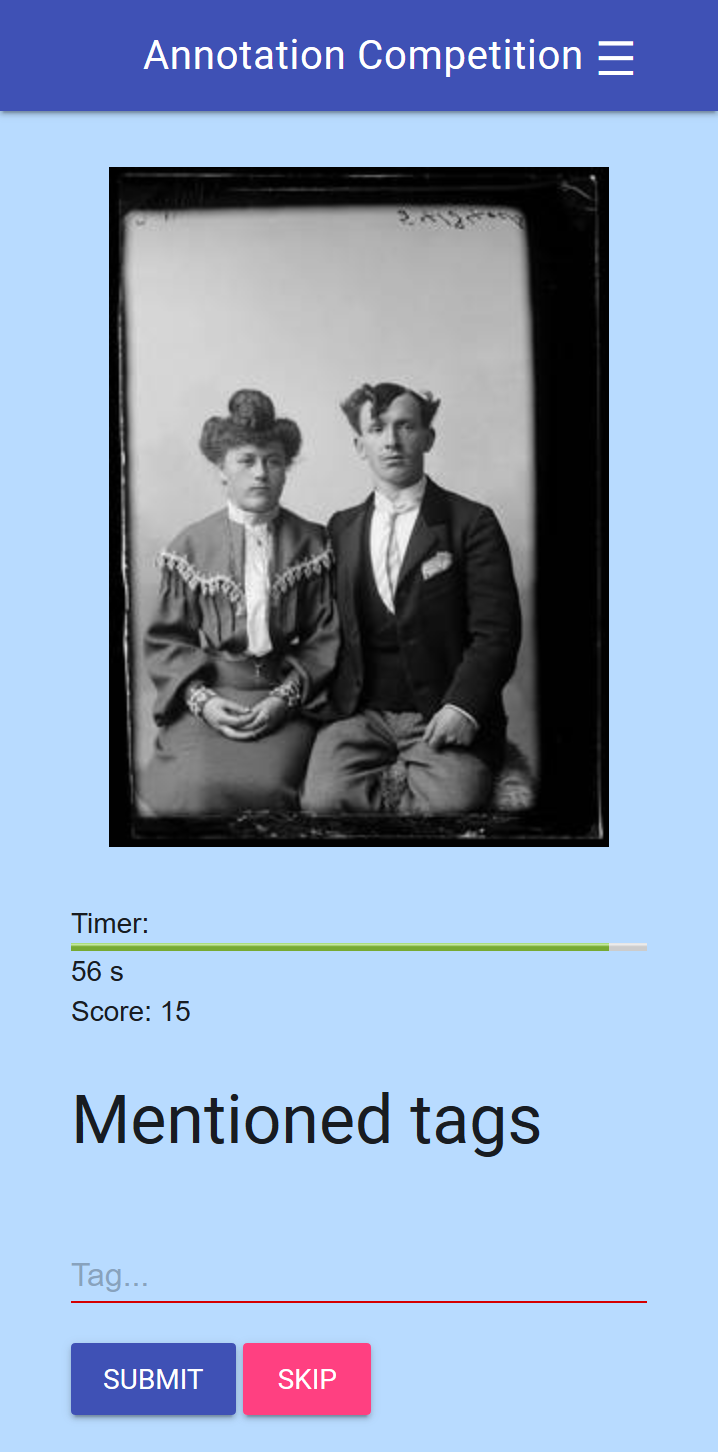
\includegraphics[width=0.45\textwidth]{gacomphs19-classic_mobile.png}
\caption{GUI for mobile devices screens, screenshot taken using Firefox and \textit{Samsung Galaxy S9} settings}
\label{gacomphs19:fig:guiclassicmobile}
\end{figure}


\subsection{Web API}
\label{gacomphs19:sec:implementation:API}
We use a JSON API to respond to dynamic requests. This includes the data and results for the game modes and form validation.
For the classic mode, a (authenticated) \texttt{GET} request to the API returns an image URL, the time limit, a list of forbidden tags and score.
A (authenticated) \texttt{POST} request should contain a JSON with a \texttt{tag} field and the entered tag. The respond will contain an accepted code, the name of the (maybe corrected) tag and the updated score.

For the cpatcha mode, a (authenticated) \texttt{GET} request to the API returns a list of image URLs, the time limit, a list of tags and the user score.
A (authenticated) \texttt{POST} request should contain a JSON with a \textit{joker} or \textit{captcha} field, together with a number. The respond will contain a selection of wrong images for the joker or the numbers of the accepted image, the correct solution and the updated score.

For the settings and the sign up form the API is used to check whether a username is available or not. You can simply \texttt{POST} the name and to get a boolean response with an error message.

Additionally, a \texttt{GET} request to the settings API returns all the data a user has contributed to (\Cref{gacomphs19:fig:webapi}).

\begin{figure}[!]
\centering
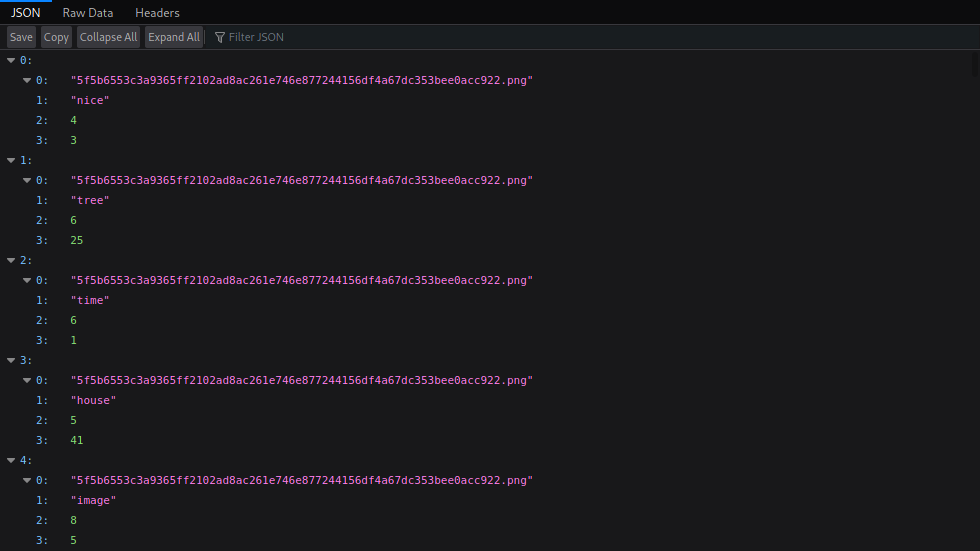
\includegraphics[width=\textwidth]{gacomphs19-image-annotation-data.png}
\caption{A typical JSON response}
\label{gacomphs19:fig:webapi}
\end{figure}
